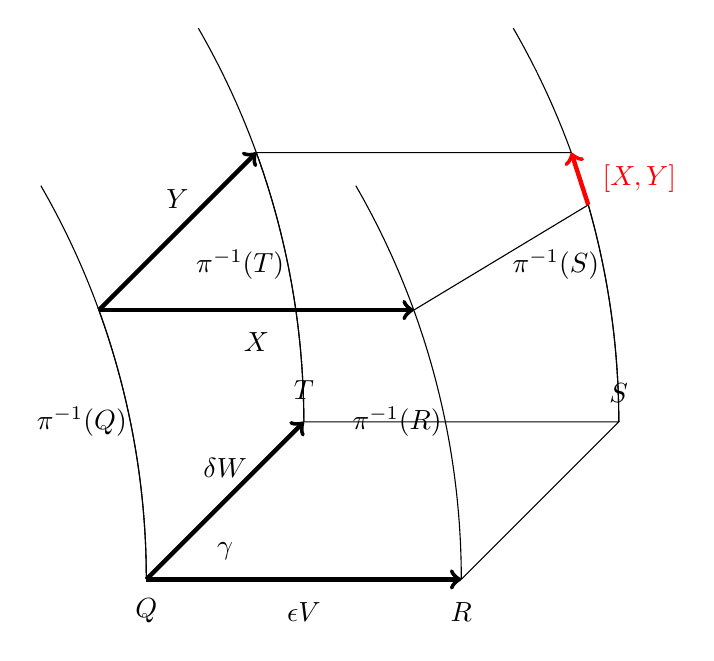
\begin{tikzpicture}[scale=2]
    \draw (0.5,0) node [label={$\gamma$}] {};
    \draw (0,0) node [label=below:{$Q$}] {};
    \draw[->, ultra thick] (0,0) -- (2,0) node [label=below:{$R$}] {} node [midway, label=below:{$\epsilon V$}] {}; % segmento Q-R
    \draw[->, ultra thick] (0,0) -- (1,1) node [label=above:{$T$}] {} node [midway, label={$\delta W$}] {}; % segmento Q-T
    \draw (1,1) -- (3,1) node [label=above:{$S$}] {} -- (2,0);

    % Fibers
    \draw (0,0) arc (0:30:5);
    \draw (2,0) arc (0:30:5);
    \draw (1,1) arc (0:30:5);
    \draw (3,1) arc (0:30:5);

    \draw (0,1) node [label=left:{$\pi^{-1}(Q)$}] {};
    \draw (2,1) node [label=left:{$\pi^{-1}(R)$}] {};
    \draw (1,2) node [label=left:{$\pi^{-1}(T)$}] {};
    \draw (3,2) node [label=left:{$\pi^{-1}(S)$}] {};

    \draw (0,0) arc (0:20:5) coordinate (pQ);
    \draw[->, ultra thick] (pQ) -- ++ (2,0) coordinate (x) node [midway, label=below:{$X$}] {};
    \draw[->, ultra thick] (pQ) -- ++(1,1) node [midway, label=above:{$Y$}] {};
    \draw (1,1) arc (0:20:5) -- ++(2,0) coordinate (z);
    \draw (3,1) arc (0:16:5) coordinate (y) ;
    \draw (x) -- (y);
    \draw[->,red,ultra thick] (y) -- (z) node [midway, label=right:{$[ X, Y]$}] {};
\end{tikzpicture}
